% Options for packages loaded elsewhere
\PassOptionsToPackage{unicode}{hyperref}
\PassOptionsToPackage{hyphens}{url}
%
\documentclass[
]{article}
\usepackage{amsmath,amssymb}
\usepackage{iftex}
\ifPDFTeX
  \usepackage[T1]{fontenc}
  \usepackage[utf8]{inputenc}
  \usepackage{textcomp} % provide euro and other symbols
\else % if luatex or xetex
  \usepackage{unicode-math} % this also loads fontspec
  \defaultfontfeatures{Scale=MatchLowercase}
  \defaultfontfeatures[\rmfamily]{Ligatures=TeX,Scale=1}
\fi
\usepackage{lmodern}
\ifPDFTeX\else
  % xetex/luatex font selection
\fi
% Use upquote if available, for straight quotes in verbatim environments
\IfFileExists{upquote.sty}{\usepackage{upquote}}{}
\IfFileExists{microtype.sty}{% use microtype if available
  \usepackage[]{microtype}
  \UseMicrotypeSet[protrusion]{basicmath} % disable protrusion for tt fonts
}{}
\makeatletter
\@ifundefined{KOMAClassName}{% if non-KOMA class
  \IfFileExists{parskip.sty}{%
    \usepackage{parskip}
  }{% else
    \setlength{\parindent}{0pt}
    \setlength{\parskip}{6pt plus 2pt minus 1pt}}
}{% if KOMA class
  \KOMAoptions{parskip=half}}
\makeatother
\usepackage{xcolor}
\usepackage[margin=1in]{geometry}
\usepackage{color}
\usepackage{fancyvrb}
\newcommand{\VerbBar}{|}
\newcommand{\VERB}{\Verb[commandchars=\\\{\}]}
\DefineVerbatimEnvironment{Highlighting}{Verbatim}{commandchars=\\\{\}}
% Add ',fontsize=\small' for more characters per line
\usepackage{framed}
\definecolor{shadecolor}{RGB}{248,248,248}
\newenvironment{Shaded}{\begin{snugshade}}{\end{snugshade}}
\newcommand{\AlertTok}[1]{\textcolor[rgb]{0.94,0.16,0.16}{#1}}
\newcommand{\AnnotationTok}[1]{\textcolor[rgb]{0.56,0.35,0.01}{\textbf{\textit{#1}}}}
\newcommand{\AttributeTok}[1]{\textcolor[rgb]{0.13,0.29,0.53}{#1}}
\newcommand{\BaseNTok}[1]{\textcolor[rgb]{0.00,0.00,0.81}{#1}}
\newcommand{\BuiltInTok}[1]{#1}
\newcommand{\CharTok}[1]{\textcolor[rgb]{0.31,0.60,0.02}{#1}}
\newcommand{\CommentTok}[1]{\textcolor[rgb]{0.56,0.35,0.01}{\textit{#1}}}
\newcommand{\CommentVarTok}[1]{\textcolor[rgb]{0.56,0.35,0.01}{\textbf{\textit{#1}}}}
\newcommand{\ConstantTok}[1]{\textcolor[rgb]{0.56,0.35,0.01}{#1}}
\newcommand{\ControlFlowTok}[1]{\textcolor[rgb]{0.13,0.29,0.53}{\textbf{#1}}}
\newcommand{\DataTypeTok}[1]{\textcolor[rgb]{0.13,0.29,0.53}{#1}}
\newcommand{\DecValTok}[1]{\textcolor[rgb]{0.00,0.00,0.81}{#1}}
\newcommand{\DocumentationTok}[1]{\textcolor[rgb]{0.56,0.35,0.01}{\textbf{\textit{#1}}}}
\newcommand{\ErrorTok}[1]{\textcolor[rgb]{0.64,0.00,0.00}{\textbf{#1}}}
\newcommand{\ExtensionTok}[1]{#1}
\newcommand{\FloatTok}[1]{\textcolor[rgb]{0.00,0.00,0.81}{#1}}
\newcommand{\FunctionTok}[1]{\textcolor[rgb]{0.13,0.29,0.53}{\textbf{#1}}}
\newcommand{\ImportTok}[1]{#1}
\newcommand{\InformationTok}[1]{\textcolor[rgb]{0.56,0.35,0.01}{\textbf{\textit{#1}}}}
\newcommand{\KeywordTok}[1]{\textcolor[rgb]{0.13,0.29,0.53}{\textbf{#1}}}
\newcommand{\NormalTok}[1]{#1}
\newcommand{\OperatorTok}[1]{\textcolor[rgb]{0.81,0.36,0.00}{\textbf{#1}}}
\newcommand{\OtherTok}[1]{\textcolor[rgb]{0.56,0.35,0.01}{#1}}
\newcommand{\PreprocessorTok}[1]{\textcolor[rgb]{0.56,0.35,0.01}{\textit{#1}}}
\newcommand{\RegionMarkerTok}[1]{#1}
\newcommand{\SpecialCharTok}[1]{\textcolor[rgb]{0.81,0.36,0.00}{\textbf{#1}}}
\newcommand{\SpecialStringTok}[1]{\textcolor[rgb]{0.31,0.60,0.02}{#1}}
\newcommand{\StringTok}[1]{\textcolor[rgb]{0.31,0.60,0.02}{#1}}
\newcommand{\VariableTok}[1]{\textcolor[rgb]{0.00,0.00,0.00}{#1}}
\newcommand{\VerbatimStringTok}[1]{\textcolor[rgb]{0.31,0.60,0.02}{#1}}
\newcommand{\WarningTok}[1]{\textcolor[rgb]{0.56,0.35,0.01}{\textbf{\textit{#1}}}}
\usepackage{graphicx}
\makeatletter
\def\maxwidth{\ifdim\Gin@nat@width>\linewidth\linewidth\else\Gin@nat@width\fi}
\def\maxheight{\ifdim\Gin@nat@height>\textheight\textheight\else\Gin@nat@height\fi}
\makeatother
% Scale images if necessary, so that they will not overflow the page
% margins by default, and it is still possible to overwrite the defaults
% using explicit options in \includegraphics[width, height, ...]{}
\setkeys{Gin}{width=\maxwidth,height=\maxheight,keepaspectratio}
% Set default figure placement to htbp
\makeatletter
\def\fps@figure{htbp}
\makeatother
\setlength{\emergencystretch}{3em} % prevent overfull lines
\providecommand{\tightlist}{%
  \setlength{\itemsep}{0pt}\setlength{\parskip}{0pt}}
\setcounter{secnumdepth}{-\maxdimen} % remove section numbering
\ifLuaTeX
  \usepackage{selnolig}  % disable illegal ligatures
\fi
\usepackage{bookmark}
\IfFileExists{xurl.sty}{\usepackage{xurl}}{} % add URL line breaks if available
\urlstyle{same}
\hypersetup{
  pdftitle={PSC4375: Interactions with Continuous Variables},
  pdfauthor={Prof.~Weldzius},
  hidelinks,
  pdfcreator={LaTeX via pandoc}}

\title{PSC4375: Interactions with Continuous Variables}
\usepackage{etoolbox}
\makeatletter
\providecommand{\subtitle}[1]{% add subtitle to \maketitle
  \apptocmd{\@title}{\par {\large #1 \par}}{}{}
}
\makeatother
\subtitle{Week 9: Lecture 14}
\author{Prof.~Weldzius}
\date{Slides Updated: 2025-03-17}

\begin{document}
\maketitle

\subsection{Interactions with Continuous
Variables}\label{interactions-with-continuous-variables}

\begin{itemize}
\tightlist
\item
  Continuing with the Michigan \textbf{social pressure get-out-the-vote
  experiment}
\item
  Create an age variable:
\end{itemize}

\begin{Shaded}
\begin{Highlighting}[]
\FunctionTok{data}\NormalTok{(social, }\AttributeTok{package=}\StringTok{"qss"}\NormalTok{)}
\NormalTok{social }\OtherTok{\textless{}{-}}\NormalTok{ social }\SpecialCharTok{\%\textgreater{}\%}
  \FunctionTok{mutate}\NormalTok{(}\AttributeTok{age =} \DecValTok{2006} \SpecialCharTok{{-}}\NormalTok{ yearofbirth)}
\FunctionTok{summary}\NormalTok{(social}\SpecialCharTok{$}\NormalTok{age)}
\end{Highlighting}
\end{Shaded}

\begin{verbatim}
##    Min. 1st Qu.  Median    Mean 3rd Qu.    Max. 
##   20.00   41.00   50.00   49.79   59.00  106.00
\end{verbatim}

\subsection{Hetergeneous effects}\label{hetergeneous-effects}

\begin{itemize}
\tightlist
\item
  From before: \pause

  \begin{itemize}
  \tightlist
  \item
    Effect of the Neighbors mailer differ from previous voters
    vs.~nonvoters?
  \item
    Used an interaction term to assess \textbf{effect heterogeneity}
    between groups
  \end{itemize}
\item
  How does the effect of the Neighbors mailer vary by age?

  \begin{itemize}
  \tightlist
  \item
    Not just two groups, but a continuum of possible age values
  \end{itemize}
\item
  Remarkable, the same \textbf{interaction term} will work here too!
\end{itemize}

\[
Y_i = \alpha + \beta_1\text{age}_i + \beta_2 \text{neighbors}_i + \beta_3 (\text{age}_i \times \text{neighbors}_i) + \varepsilon_i
\]

\subsection{Predicted values from non-interacted
model}\label{predicted-values-from-non-interacted-model}

\begin{itemize}
\tightlist
\item
  Let \(X_i =\) age\(_i\) and \(Z_i =\) neighbors\(_i\)
\end{itemize}

\[
\hat{Y}_i = \hat{\alpha} + \hat{\beta}_1 X_i + \hat{\beta}_2 Z_i 
\]

\begin{center}
\begin{tabular}{ r | l  l }
 & Control ($Z_i = 0$) & Neighbors ($Z_i = 1$) \\
\hline
25 year-old ($X_i = 25$)  & $\hat{\alpha} + \hat{\beta}_1 25$ &  $\hat{\alpha} + \hat{\beta}_1 25 + \hat{\beta}_2$ \\
26 year-old ($X_i = 26$) & $\hat{\alpha} + \hat{\beta}_1 26$ &  $\hat{\alpha} + \hat{\beta}_1 26 + \hat{\beta}_2$\\
\end{tabular}
\end{center}

\begin{itemize}
\item Effect of Neighbors for a 25 year-old:
\end{itemize}\vspace{-5pt}

\[
(\hat{\alpha} + \hat{\beta}_1 25 + \hat{\beta}_2) - (\hat{\alpha} + \hat{\beta}_1 25) = \hat{\beta}_2
\]

\vspace{-5pt}

\begin{itemize}
\item Effect of Neighbors for a 26 year-old:
\end{itemize}\vspace{-5pt}

\[
(\hat{\alpha} + \hat{\beta}_1 26 + \hat{\beta}_2) - (\hat{\alpha} + \hat{\beta}_1 26) = \hat{\beta}_2
\]

\subsection{Visualizing the
regression}\label{visualizing-the-regression}

\includegraphics{psc4375_lecture_14_slides_code_files/figure-latex/unnamed-chunk-3-1.pdf}

\subsection{Visualizing the
regression}\label{visualizing-the-regression-1}

\includegraphics{psc4375_lecture_14_slides_code_files/figure-latex/unnamed-chunk-4-1.pdf}

\subsection{Visualizing the
regression}\label{visualizing-the-regression-2}

\includegraphics{psc4375_lecture_14_slides_code_files/figure-latex/unnamed-chunk-5-1.pdf}

\subsection{Predicted values from interacted
model}\label{predicted-values-from-interacted-model}

\[
\hat{Y}_i = \hat{\alpha} + \hat{\beta}_1 X_i + \hat{\beta}_2 Z_i + \hat{\beta}_3  X_i Z_i
\]

\begin{center}
\begin{tabular}{ r | l  l }
 & Control ($Z_i = 0$) & Neighbors ($Z_i = 1$) \\
\hline
25 year-old ($X_i = 25$)  & $\hat{\alpha} + \hat{\beta}_1 25$ &  $\hat{\alpha} + \hat{\beta}_1 25 + \hat{\beta}_2\ + \hat{\beta}_3 25$ \\
26 year-old ($X_i = 26$) & $\hat{\alpha} + \hat{\beta}_1 26$ &  $\hat{\alpha} + \hat{\beta}_1 26 + \hat{\beta}_2 + \hat{\beta}_2\ + \hat{\beta}_3 26$ \\
\end{tabular}
\end{center}

\begin{itemize}
\tightlist
\item
  Effect of Neighbors for a 25 year-old: \vspace{-10pt}
\end{itemize}

\[
(\hat{\alpha} + \hat{\beta}_1 25 + \hat{\beta}_2 + \hat{\beta}_3 25) - (\hat{\alpha} + \hat{\beta}_1 25) = \hat{\beta}_2 + \hat{\beta}_3 25)
\]

\begin{itemize}
\tightlist
\item
  Effect of Neighbors for a 26 year-old: \vspace{-10pt}
\end{itemize}

\[
(\hat{\alpha} + \hat{\beta}_1 26 + \hat{\beta}_2 + \hat{\beta}_3 26) - (\hat{\alpha} + \hat{\beta}_1 26) = \hat{\beta}_2 + \hat{\beta}_3 26)
\]

\begin{itemize}
\tightlist
\item
  Effect of Neighbors for a \(x\) year-old: \vspace{-10pt}
\end{itemize}

\[
\hat{\beta}_2 + \hat{\beta}_3 x
\]

\subsection{Visualizing the
interaction}\label{visualizing-the-interaction}

\includegraphics{psc4375_lecture_14_slides_code_files/figure-latex/unnamed-chunk-6-1.pdf}

\subsection{Interpretting
coefficients}\label{interpretting-coefficients}

\[
Y_i = \alpha + \beta_1\text{age}_i + \beta_2 \text{neighbors}_i + \beta_3 (\text{age}_i \times \text{neighbors}_i)
\]

\begin{itemize}
\tightlist
\item
  \(\hat{\alpha}\): average turnout for 0 year-olds in the control
  group.
\item
  \(\hat{\beta}_1\): slope of regression line for age in the control
  group.
\item
  \(\hat{\beta}_2\): average effect of Neighbors mailer for 0 year-olds.
\item
  \(\hat{\beta}_3\): change in the \textbf{effect} of the Neighbors
  mailer for a 1-year \(\uparrow\) in age.

  \begin{itemize}
  \tightlist
  \item
    Effect for \(x\) year-olds: \(\hat{\beta}_2 + \hat{\beta}_3 x\)
  \item
    Effect for \((x+1)\) year-olds:
    \(\hat{\beta}_2 + \hat{\beta}_3 (x+1)\)
  \item
    Change in effect: \(\hat{\beta}_3\)
  \end{itemize}
\end{itemize}

\subsection{Interactions in R}\label{interactions-in-r}

\begin{itemize}
\tightlist
\item
  You can use the \texttt{:} way to create interaction terms like last
  time:
\end{itemize}

\begin{Shaded}
\begin{Highlighting}[]
\NormalTok{int.fit }\OtherTok{\textless{}{-}} \FunctionTok{lm}\NormalTok{(primary2006 }\SpecialCharTok{\textasciitilde{}}\NormalTok{ age }\SpecialCharTok{+}\NormalTok{ neighbors }\SpecialCharTok{+}\NormalTok{ age}\SpecialCharTok{:}\NormalTok{neighbors, }\AttributeTok{data =}\NormalTok{ social.neighbor)}
\FunctionTok{coef}\NormalTok{(int.fit)}
\end{Highlighting}
\end{Shaded}

\begin{verbatim}
##   (Intercept)           age     neighbors age:neighbors 
##  0.2680512150  0.0001846143  0.0873583626 -0.0003345028
\end{verbatim}

\begin{itemize}
\tightlist
\item
  Or you can use the \texttt{var1\ *\ var2} shortcut, which will add
  both variable and their interaction:
\end{itemize}

\begin{Shaded}
\begin{Highlighting}[]
\NormalTok{int.fit2 }\OtherTok{\textless{}{-}} \FunctionTok{lm}\NormalTok{(primary2006 }\SpecialCharTok{\textasciitilde{}}\NormalTok{ age}\SpecialCharTok{*}\NormalTok{neighbors, }\AttributeTok{data =}\NormalTok{ social.neighbor)}
\FunctionTok{coef}\NormalTok{(int.fit2)}
\end{Highlighting}
\end{Shaded}

\begin{verbatim}
##   (Intercept)           age     neighbors age:neighbors 
##  0.2680512150  0.0001846143  0.0873583626 -0.0003345028
\end{verbatim}

\subsection{General interpretation of
interactions}\label{general-interpretation-of-interactions}

\[
\hat{Y}_i = \hat{\alpha} + \hat{\beta}_1 X_i + \hat{\beta}_2 Z_i + \hat{\beta}_3  X_i Z_i
\]

\begin{itemize}
\tightlist
\item
  \(\hat{\alpha}\): average turnout when \(X_i\) and \(Z_i\) are \(0\).

  \begin{itemize}
  \tightlist
  \item
    \(\hat{\beta}_1\): average change in \(Y_i\) of a one-unit change in
    \(X_i\) when \(Z_i = 0\).
  \item
    \(\hat{\beta}_2\): average change in \(Y_i\) of a one-unit change in
    \(Z_i\) when \(X_i = 0\).
  \item
    \(\hat{\beta}_3\): has two equivalent interpretations:

    \begin{itemize}
    \tightlist
    \item
      Change in the effect/slope of \(X_i\) for a one-unit change in
      \(Z_i\)
    \item
      Change in the effect/slope of \(Z_i\) for a one-unit change in
      \(X_i\)
    \end{itemize}
  \end{itemize}
\end{itemize}

\subsection{Nonlinear relationships}\label{nonlinear-relationships}

\begin{figure}
\centering
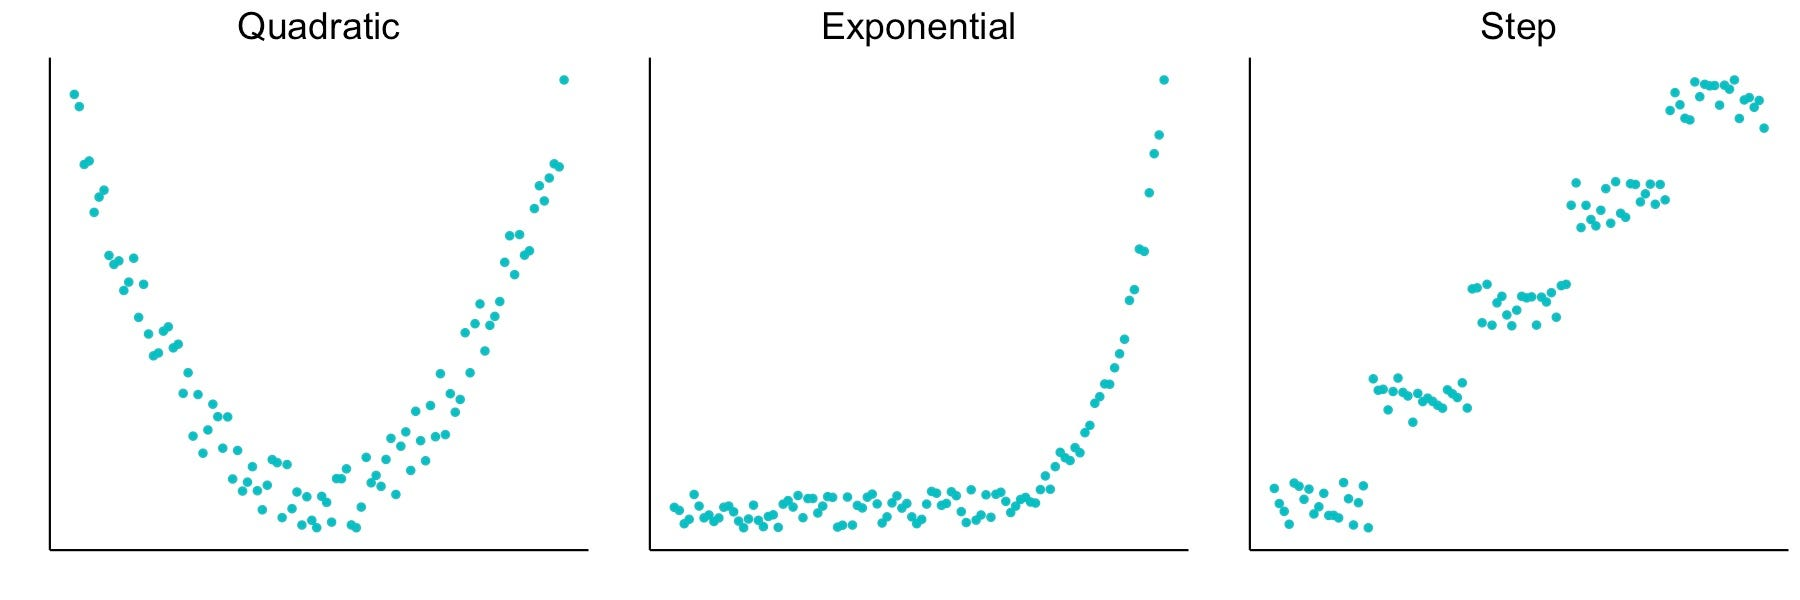
\includegraphics{figs/nonlinear.jpg}
\caption{Types of Non-linear Relationships}
\end{figure}

\subsection{Linear regression are
linear}\label{linear-regression-are-linear}

\[
\hat{Y}_i = \hat{\alpha} + \hat{\beta}_1 X_i
\]

\begin{itemize}
\tightlist
\item
  Standard linear regression can only pick up \textbf{linear}
  relationships.
\item
  What if the relationship between \(X_i\) and \(Y_i\) is nonlinear?
\end{itemize}

\subsection{Adding a squared term}\label{adding-a-squared-term}

\begin{itemize}
\tightlist
\item
  To allow for nonlinearity in age, add a squared term to the model
\end{itemize}

\[
\hat{Y}_i = \hat{\alpha} + \hat{\beta}_1 \text{age}_i + \hat{\beta}_2 \text{age}_i^2
\]

\begin{itemize}
\tightlist
\item
  We are now fitting a \textbf{parabola} to the data.
\item
  In R, we need to wrap the squared term in \texttt{I()}:
\end{itemize}

\begin{Shaded}
\begin{Highlighting}[]
\NormalTok{fit.sq }\OtherTok{\textless{}{-}} \FunctionTok{lm}\NormalTok{(primary2006 }\SpecialCharTok{\textasciitilde{}}\NormalTok{ age }\SpecialCharTok{+} \FunctionTok{I}\NormalTok{(age}\SpecialCharTok{\^{}}\DecValTok{2}\NormalTok{), }\AttributeTok{data =}\NormalTok{ social)}
\FunctionTok{coef}\NormalTok{(fit.sq)}
\end{Highlighting}
\end{Shaded}

\begin{verbatim}
##   (Intercept)           age      I(age^2) 
## -8.168043e-02  1.227357e-02 -8.078954e-05
\end{verbatim}

\begin{itemize}
\tightlist
\item
  \(\hat{\beta}_2\): how the effect of age increases as age increases
\end{itemize}

\subsection{Predicted values from lm()}\label{predicted-values-from-lm}

\begin{itemize}
\tightlist
\item
  We can get predicted values out of R using the \texttt{predict()}
  function:
\end{itemize}

\begin{Shaded}
\begin{Highlighting}[]
\FunctionTok{predict}\NormalTok{(fit.sq, }\AttributeTok{newdata =} \FunctionTok{list}\NormalTok{(}\AttributeTok{age =} \FunctionTok{c}\NormalTok{(}\DecValTok{20}\NormalTok{, }\DecValTok{21}\NormalTok{, }\DecValTok{22}\NormalTok{)))}
\end{Highlighting}
\end{Shaded}

\begin{verbatim}
##         1         2         3 
## 0.1314752 0.1404364 0.1492361
\end{verbatim}

\begin{itemize}
\tightlist
\item
  Create a vector of ages to predict and save predictions:
\end{itemize}

\begin{Shaded}
\begin{Highlighting}[]
\NormalTok{age.vals }\OtherTok{\textless{}{-}} \DecValTok{20}\SpecialCharTok{:}\DecValTok{85}
\NormalTok{age.preds }\OtherTok{\textless{}{-}} \FunctionTok{predict}\NormalTok{(fit.sq, }\AttributeTok{newdata =} \FunctionTok{list}\NormalTok{(}\AttributeTok{age =}\NormalTok{ age.vals))}
\NormalTok{age.plot }\OtherTok{\textless{}{-}} \FunctionTok{tibble}\NormalTok{(age.vals,age.preds)}
\end{Highlighting}
\end{Shaded}

\begin{itemize}
\tightlist
\item
  Plot the predictions:
\end{itemize}

\begin{Shaded}
\begin{Highlighting}[]
\FunctionTok{ggplot}\NormalTok{(age.plot,}\FunctionTok{aes}\NormalTok{(}\AttributeTok{x =}\NormalTok{ age.vals, }\AttributeTok{y =}\NormalTok{ age.preds)) }\SpecialCharTok{+}
  \FunctionTok{geom\_point}\NormalTok{(}\AttributeTok{color =} \StringTok{"blue"}\NormalTok{, }\AttributeTok{size =} \DecValTok{3}\NormalTok{, }\AttributeTok{shape =} \DecValTok{1}\NormalTok{) }\SpecialCharTok{+} \FunctionTok{ylim}\NormalTok{(}\FloatTok{0.1}\NormalTok{, }\FloatTok{0.55}\NormalTok{) }\SpecialCharTok{+}
  \FunctionTok{labs}\NormalTok{(}\AttributeTok{x =} \StringTok{"Age"}\NormalTok{, }\AttributeTok{y =} \StringTok{"Predicted Turnout Rate"}\NormalTok{) }\SpecialCharTok{+} \FunctionTok{theme\_bw}\NormalTok{()}
\end{Highlighting}
\end{Shaded}

\section{Plotting predicted values}\label{plotting-predicted-values}

\includegraphics{psc4375_lecture_14_slides_code_files/figure-latex/unnamed-chunk-13-1.pdf}

\subsection{Plotting lines instead of
points:}\label{plotting-lines-instead-of-points}

\begin{itemize}
\tightlist
\item
  If you want to connect the dots in your scatterplot, you can use
  \texttt{geom\_line()}:
\end{itemize}

\begin{Shaded}
\begin{Highlighting}[]
\FunctionTok{ggplot}\NormalTok{(age.plot, }\FunctionTok{aes}\NormalTok{(}\AttributeTok{x =}\NormalTok{ age.vals, }\AttributeTok{y =}\NormalTok{ age.preds)) }\SpecialCharTok{+}
  \FunctionTok{geom\_line}\NormalTok{(}\AttributeTok{color =} \StringTok{"blue"}\NormalTok{, }\AttributeTok{size =} \FloatTok{1.5}\NormalTok{) }\SpecialCharTok{+}
  \FunctionTok{ylim}\NormalTok{(}\FloatTok{0.1}\NormalTok{, }\FloatTok{0.55}\NormalTok{) }\SpecialCharTok{+}
  \FunctionTok{labs}\NormalTok{(}\AttributeTok{x =} \StringTok{"Age"}\NormalTok{, }\AttributeTok{y =} \StringTok{"Predicted Turnout Rate"}\NormalTok{) }\SpecialCharTok{+}
  \FunctionTok{theme\_bw}\NormalTok{()}
\end{Highlighting}
\end{Shaded}

\subsection{Plotting predicted
values}\label{plotting-predicted-values-1}

\begin{itemize}
\tightlist
\item
  If you want to connect the dots in your scatterplot, you can use
  \texttt{geom\_line()}:
\end{itemize}

\includegraphics{psc4375_lecture_14_slides_code_files/figure-latex/unnamed-chunk-15-1.pdf}

\subsection{Comparing to linear fit}\label{comparing-to-linear-fit}

\begin{itemize}
\tightlist
\item
  If you want to connect the dots in your scatterplot, you can use
  \texttt{geom\_line()}:
\end{itemize}

\includegraphics{psc4375_lecture_14_slides_code_files/figure-latex/unnamed-chunk-16-1.pdf}

\subsection{Diagnosing nonlinearity}\label{diagnosing-nonlinearity}

\begin{itemize}
\tightlist
\item
  One independent variable: just look at a scatterplot.
\item
  With multiple independent variables, harder to diagnose.
\item
  One useful tool: scatterplot of residuals versus independent
  variables.
\item
  Example: let's talk about walking and health
\end{itemize}

\begin{Shaded}
\begin{Highlighting}[]
\NormalTok{health }\OtherTok{\textless{}{-}} \FunctionTok{read.csv}\NormalTok{(}\StringTok{"../data/health.csv"}\NormalTok{)}

\NormalTok{w.fit }\OtherTok{\textless{}{-}} \FunctionTok{lm}\NormalTok{(weight }\SpecialCharTok{\textasciitilde{}}\NormalTok{  steps.lag }\SpecialCharTok{+}\NormalTok{ dayofyear, }\AttributeTok{data =}\NormalTok{ health)}
\end{Highlighting}
\end{Shaded}

\subsection{Residual plot}\label{residual-plot}

\includegraphics{psc4375_lecture_14_slides_code_files/figure-latex/unnamed-chunk-19-1.pdf}

\subsection{Add a squared term for a better
fit}\label{add-a-squared-term-for-a-better-fit}

\begin{Shaded}
\begin{Highlighting}[]
\NormalTok{w.fit.sq }\OtherTok{\textless{}{-}} \FunctionTok{lm}\NormalTok{(weight }\SpecialCharTok{\textasciitilde{}}\NormalTok{ steps.lag }\SpecialCharTok{+}\NormalTok{ dayofyear }\SpecialCharTok{+} \FunctionTok{I}\NormalTok{(dayofyear}\SpecialCharTok{\^{}}\DecValTok{2}\NormalTok{), }\AttributeTok{data =}\NormalTok{ health)}
\FunctionTok{coef}\NormalTok{(w.fit.sq)}
\end{Highlighting}
\end{Shaded}

\begin{verbatim}
##    (Intercept)      steps.lag      dayofyear I(dayofyear^2) 
##   1.749194e+02  -2.509427e-03  -5.288116e-02   1.439635e-04
\end{verbatim}

\subsection{Residual plot, redux}\label{residual-plot-redux}

\includegraphics{psc4375_lecture_14_slides_code_files/figure-latex/unnamed-chunk-21-1.pdf}

\end{document}
